\documentclass[12pt]{article}
\usepackage{amssymb,amsfonts,amsthm,mathtools,float,color}
\usepackage{caption,subcaption,tikz,gensymb,pgfplots}
\usepackage{graphicx}
\graphicspath{ {images/} }
\usepackage[]{algorithm2e}
\pgfplotsset{compat = newest}
\DeclarePairedDelimiter\ceil{\lceil}{\rceil}
\DeclarePairedDelimiter\floor{\lfloor}{\rfloor}
\usepackage[hmargin=1in,vmargin=1in]{geometry}
\newcommand{\si}{\sigma}
\DeclareMathOperator{\lb}{lb}
\DeclareMathOperator{\ls}{ls}
\DeclareMathOperator{\rb}{rb}
\DeclareMathOperator{\rs}{rs}
\DeclareMathOperator{\LB}{LB}
\DeclareMathOperator{\Max}{Max}
\DeclareMathOperator{\LS}{LS}
\DeclareMathOperator{\RB}{RB}
\DeclareMathOperator{\RS}{RS}
\DeclareMathOperator{\hook}{hook}
      \theoremstyle{plain}
      \newtheorem{theorem}{Theorem}[section]
      \newtheorem{lemma}[theorem]{Lemma}
      \newtheorem{corollary}[theorem]{Corollary}
      \newtheorem{proposition}[theorem]{Proposition}
      \theoremstyle{definition}
      \newtheorem{definition}[theorem]{Definition}
      \theoremstyle{remark}
      \newtheorem{remark}[theorem]{Remark}
      \theoremstyle{plain}
      \newtheorem{conjecture}{Conjecture}[section]
\def\vs{\vspace{1\baselineskip}}
\def\svs{\vspace{.5\baselineskip}}
\def\bs{\vspace{5\baselineskip}}
\def\zik{\mathcal{Z}_{i,k}}
\def\setzik{\{\mathcal{Z}\}_k}
\def\Z{\mathcal{Z}}
%\newcommand{\tre}[1]{\textcolor{red}{}}
\newcommand{\tre}{\textcolor{red}}
\newcommand{\tbl}[1]{\textcolor{blue}{}}
\newcommand{\tgr}[1]{\textcolor{green}{}}
\DeclareMathOperator{\WLB}{WLB}
\DeclareMathOperator{\WLS}{WLS}
\DeclareMathOperator{\WRB}{WRB}
\DeclareMathOperator{\WRS}{WRS}
\DeclareMathOperator{\WF}{WF}
\DeclareMathOperator{\W}{\mathcal{W}}
\def\zik{\mathcal{Z}_{i,k}}
\def\setzik{\{\mathcal{Z}\}_k}
\def\Z{\mathcal{Z}}
\def\M{{\bf M}}
\def\l{\ell}
\def\multiset#1#2{\ensuremath{\left(\kern-.3em\left(\genfrac{}{}{0pt}{}{#1}{#2}\right)\kern-.3em\right)}}
\newcommand{\Rtil}{\widetilde{R}}
\newcommand{\LBtil}{\widetilde{\LB}}
\newcommand{\LStil}{\widetilde{\LS}}
\newcommand{\RBtil}{\widetilde{\RB}}
\newcommand{\RStil}{\widetilde{\RS}}
\newcommand{\gauss}[2]{\genfrac{[}{]}{0pt}{}{#1}{#2}} 
\newcommand{\TODO}{\tre{TODO!!!!!!}}
\newcommand{\interesting}{\tre{SUPER INTERESTING\\}}
\newcommand{\figureout}{\tre{Need to figure this out\\}}
\newcommand{\N}{\mathbb{N}}

\begin{document}
\title{Playing Pong with Deep Reinforcement Learning}
\author{Bobby Dorward, Ryan Wilson, and Eric Bell}
\maketitle

\section{Introduction and Background}
%type here
%percent signs are comments
%type \section{section_name} for a new section
%compile to see what it looks like
\par 
The history between artificial intelligence and gaming is long standing because short term choices give rise to long term sophistication.  For example, the moves possible in the game of Go are few, yet it took one of the most sophisticated machine learning algorithms to date to be able to perform sufficiently at this problem.  AlphaGo is but one of the few applications of deep neural networks that have. We aim to revisit this relationship between machine learning and gaming in order to gain facility with how machine learning, specifically deep neural networks, are used.
\par
We have trained our neural network through reinforcement learning, specifically through an implementation of deep $Q$-learning \cite{deepatari}. In $Q$-learning, we try to approximate the function $Q(s_i,a)$, which represents the expected value of taking action $a$ on state $s_i$. At optimality, $Q^*$ should obey the Bellman equation $$Q^*(s_i,a) = r_i + \gamma \max_{a'}Q^*(s_{i+1},a'),$$
where $r_i$ is the immediate reward from performing action $a$ on state $s_i$ and $\gamma$ is a discount factor. We can use the Bellman equation to iteratively try to approximate $Q$. More specifically, when training the neural network, we use the Bellman equation to create our loss function. The pseudocode can be found in Algorithm~\ref{qlearning}. 

We implement a technique called experience replay, which means that we save all the data needed to train the neural network and then randomly sample from these memories to train the network. This gives the advantage that we training on memories that are not correlated and can hopefully get out of local mins. In addition, we can train multiple times on each memory and so we get more use out of each observed result.


\begin{figure}
\begin{algorithm}[H]
\caption{The deep $Q$-learning algorithm}\label{qlearning}
\vspace{20pt}
Predict optimal action $a$ by feeding difference frame $x_i$ into neural network\\
Take action $a$, observe reward $r$ and set $m=\max_{a'} Q(x_{i+1},a)$\\
Save $(x_i, a,r, m)$ as a memory for experience replay\\
Randomly sample memories and use these to train the neural network on the loss function $(r+\gamma m-Q(x_i,a))^2$.

\vspace{20pt}
\end{algorithm}
\end{figure}

%[BOBBY PLS WRITE THIS SECTION SO ITS THE MATHINESS YOU WANT]
\par
Our algorithm interacts with the game through the OpenAI Gym \cite{openai}, an environment that allows the programmer to interact with Atari games (as well as a few other simulations) such that a machine learning algorithm can be trained to play the game (``solve" the problem).  What this entails is that the Gym allows us to extract pixel data from the game, signal actions for the AI to take on a frame-by-frame basis, and collect feedback used to train the algorithm.  Our original goal when starting this project was to apply this network to the ``DoomBasic-v0" \cite{doom} but due to limitations, we decided to start with the simpler ``Pong-v0" \cite{pong} environment.  This environment runs a typical game of pong: a ball bounces between two paddles and one player scores when the ball hits the opposing side of the screen.  The two players continue until someone scores 21 points, after which the game ends.
\section{Data}
\par
As previously mentioned, the data we used as input into our deep network was the pixel data of the environment.  Each pixel is represented as an array of three elements, representing the three channels of an RGB pixel, and these pixels are passed into the neural network as inputs.  Neural networks by nature are memory-intensive data structures due to the large amount of nodes and connections they contain.  This is especially true when one uses a more complex version of a neural network, such as the deep neural networks we have implemented.  Therefore, despite our best efforts to make our implementation generic and applicable to many different environments, we had to make pong-specific alterations to our data to streamline the size of the network and make it runnable on the resources we had available to us.
\par
The first change we made was to grayscale the pixel values, thereby cutting the data we need to put into our network by a factor of three.  Essentially what this means is that we have averaged the three values of the RGB channel into one value for each pixel.  Next, we cropped the data being given to us by the OpenAI Gym in order to exclude all the pixels on the screen that weren't directly relevant to the frame-by-frame progression of the game.  The scoreboard, the white edges, and the padding behind each paddle was cropped to minimize the input count of the network.  Through this preprocessing, we were able to reduce the amount of inputs being taken for each frame to 20,800.
%(Downsampling/Pooling?) 
\par
Finally, since the game of pong does not consist of still images, but rather gains meaning through the motion of the game objects (two paddles and the ball), we needed to capture this motion using the pixel data.  We achieve this by extrapolating a difference frame (suggested in \cite{karpathy}), shown in Figure~\ref{image}, between each subsequent pair of images, in which we subtract the first image from the second image.  Through this, we can train the algorithm with data that represents where the game objects have been and where they're going, zeroing out any unmoving (and thus irrelevant) pixels in the process.  It is because of these difference frames that we have limited the action that our AI can take; instead of the 5 actions that are available by default to the algorithm, we've limited it to only moving left and right.  This way, the algorithm is always able to see its own paddle because it's constantly in motion and therefore creating data on the difference frame.\newline
\begin{figure}[h]
\centering
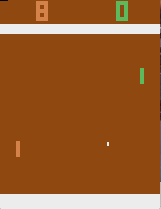
\includegraphics[scale=.9]{env.png}
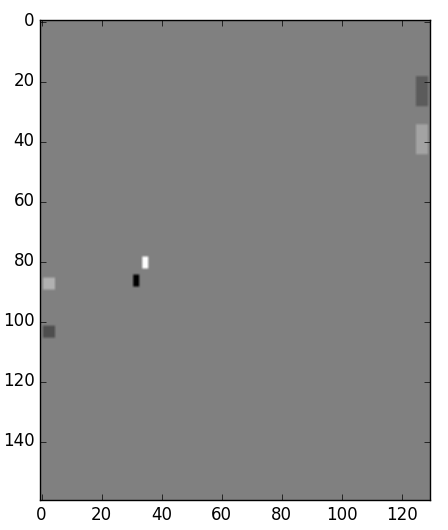
\includegraphics[scale=0.5]{df.png}
\newline
\centering
\caption{Raw data (left) and preprocessed difference frame (right) used as input into the neural network}\label{image}
\end{figure}
\section{Implementation}
\par
Our deep network is implemented in a python 3 program called ``deep\_pong.py", which is dependent on the OpenAI Gym module, numpy, and Tensorflow \cite{tensorflow}, a package developed by Google that constructs and trains neural networks.  We used the code in \cite{medium,tutorial} as a jumping-off point to try to understand $Q$-learning, though we made extensive changes to the code. The program starts by defining the topology and hyperparameters used to train the neural network.  The learning rate starts at 1e-7 and decays to 1e-8 by multiplying the current rate by .999 every training session.  We then define epsilon as 1, a probability that a random action will be taken, which ensures that the AI will receive positive reward simply by pure chance, and define epsilon's decay as .999992, which is multiplied by the current epsilon during every training session.  The next value is the discount multiplier for expected future reward ($\gamma$ in $Q$-learning).  We introduce two discounted factors to take advantage of previous knowledge about pong. We know that we will only get a nonzero reward after one of the sides scores. Therefore we decided not to immediately store memories after observing them, but to wait until someone had scored, at which point we could use one of the discount factors to ensure that we were always training on nonzero rewards. The other discount factor is used for the actual $Q$-learning algorithm.

 We then define the maximum episode count (20000, a count we'd have to run for over a week to reach), and the batch size, which corresponds to the amount of instances being sampled to train the network during each session of training.  After establishing a mechanism for saving the neural network and defining a few functions that will help us construct the model and preprocess the data, we then construct the neural network using Tensorflow.
\par
Our deep neural network consists of 20800 input nodes feeding into two fully connected hidden layers, the first layer having 100 nodes and the second layer having 50 nodes, which then feed into two output nodes corresponding to the two actions (right and left).  The weights are initialized corresponding to a normal distribution with a standard deviation of 0.1, and the bias is initialized to 0.3.  We define our loss function as minimization of the sum of squares difference between the Q value given by the neural network and the Q value predicted by the Bellman equation. We then multiply this by a one-hot vector of the action taken to ensure weights are only altered for the action taken. We use stochastic gradient descent as the optimizer.  Since the model for the neural network is now established, we can then initialize the model and start the OpenAI Gym environment.
\par
The first thing we do when running the Tensorflow session is try to load a previously made model and restore the weights if possible (code found in \cite{greydanus}).  After that, we create the good and bad memory lists, where the memories collected in a point will be stored depending on whether they lead to a positive or negative reward. This was done because the original $Q$-learning algorithm had the model training on almost exclusively negative rewards, which caused the weights of the network to diverge to negative infinity.  On the start of a new game, a first random action is chosen to allow the creation of a first difference frame, the first frame is preprocessed and the memory lists for the current game are created.  For each frame following, an action is chosen either based on randomness if a random float is higher than epsilon, or otherwise is based on what action leads to the highest Q.  The state derived from taking that action is then saved so that future expected reward can be calculated later.  If the frame resulted in the scoring of a point or the game being over, then the memories collected during the run are assigned target Q values based on the outcome of the point and stored in either the good or bad memories lists based on the sign of the reward.  Old memories are overwritten if the list size exceeds the memory size defined previously (40000 in our case).  Finally, after all the memories have been stored, we can begin training.  In order to train, the memories (instances) are sampled at random from the list of good and bad memories according to the specified batch size.  Two times the amount of memory that just happened (good if we got a point, bad if they got a point) is passed into the network, which then results in the adjustments of the network's weights through minimization of the loss function defined earlier. This was done to try to break out of local mins caused by training equally on good and bad memories, i.e., the vast majority of memories are bad and so sampling equally on good and bad memories was leading to the network overvaluing the experiences from the good memories and getting stuck in the local mins of wiggling around one of the boundaries.
\section{Results and Discussion}
\par 
Despite much effort, our algorithm is not performing as expected: the large majority of games played by our algorithm end in scoreless losses.  This could partially be due to a lack of exploration of the hyperparameter landscape: due to technical limitations, training time was too long to adequately evaluate the performance of a neural network with each possible configuration.  Initially, training time was prohibitively slow even on very simple models; however, in order to fix this problem we prepared tensorflow to run on a desktop GPU. This was highly effective, but involved many hours of work, including some editing of the BIOS initialization script on the desktop, the installation of a new operating system, extensive driver-related troubleshooting, and numerous crashes.  Since the GPU speedup was first successfully executed, the desktop has been running almost nonstop (barring some crashes) in order to test hyperparameters. However, even in spite of this the technical limitations put a cap on how large of a network we could generate without running out of memory, and our topology reflects this upper limit.  It's possible that even though we have a large number of nodes, it's still insufficient to handle the massive amounts of input generated by the environment.
\par
However, our difficulties are also partially due to the realization of pong in OpenAI Gym's environment.  The environment has your AI faced against a premade AI that is quite good at returning shots.  One particular facet of the AI that has posed problems for learning is its service pattern, which alternates between one of two spots (one on top, one on bottom) depending on whether the player returned the serve or not.  Due to this pattern, we could see our algorithm learning to start by moving to either the very top and very bottom of the screen and then struggle to learn to move to the other side after several points of missing the ball, which was being served in the same spot on the other side of the screen.  We tried to alleviate this by suppressing the learning rate and implementing a decaying learning rate that would hopefully minimize the effect these service problems had on the weights it learned during earlier training sessions.  Ideally, if we had the ability to alter the environment provided to us by the OpenAI Gym we would have pitted our algorithm against a more fair opponent: itself.  At the very least, altering the service pattern so that it served in a random direction rather than in the same direction every time would have potentially allowed for our algorithm to learn more easily.
\par
The ``Pong-v0" environment is not an impossible problem, and as a matter of fact, there exist several implementations that work well on the webpage of the problem \cite{pong}, but the difference between these implementations and our own is that the neural networks they used were more sophisticated than what our computational resources could handle.  For example, one of the solutions uses a convolutional neural network \cite{eval,conv}, and while we attempted to train one of these networks, training time was incredibly slow (~1.5 minutes for 1 iterations, which translates to 2.5 hours for 100 iterations), and creating a network of any significant size resulted in running out of memory.  In summary, in order for success to be achieved on this project, either we needed to alter the problem (opposing player AI), or gain access to more computational resources, such as the supercomputer.
\begin{figure}
\begin{center}
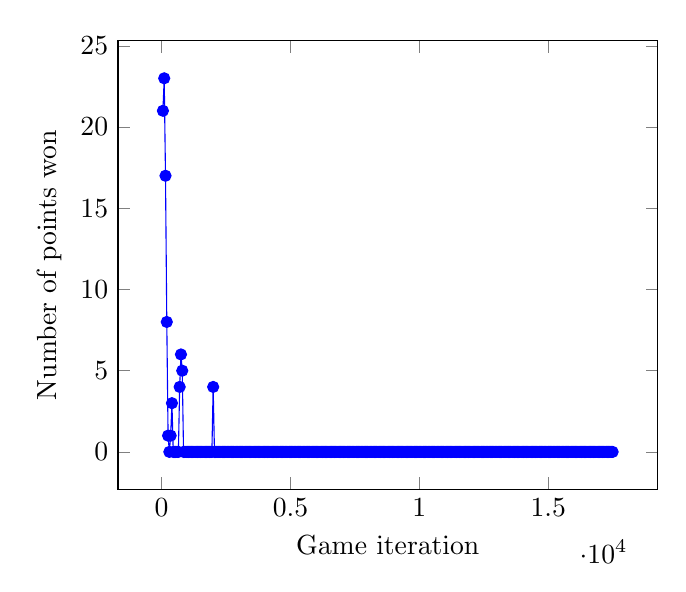
\begin{tikzpicture}
\begin{axis}[
xlabel = Game iteration,
ylabel=Number of points won,
legend pos = south east,
scaled y ticks = false,
yticklabel style={/pgf/number format/fixed,
                     /pgf/number format/precision=3},
]

\addplot[color=blue,
mark=*,
] 
coordinates { %replace the coordinates here (x,y)
(50,21)
(100,23)
(150,17)
(200,8)
(250,1)
(300,0)
(350,1)
(400,3)
(450,0)
(500,0)
(550,0)
(600,0)
(650,0)
(700,4)
(750,6)
(800,5)
(850,0)
(900,0)
(950,0)
(1000,0)
(1050,0)
(1100,0)
(1150,0)
(1200,0)
(1250,0)
(1300,0)
(1350,0)
(1400,0)
(1450,0)
(1500,0)
(1550,0)
(1600,0)
(1650,0)
(1700,0)
(1750,0)
(1800,0)
(1850,0)
(1900,0)
(1950,0)
(2000,4)
(2050,0)
(2100,0)
(2150,0)
(2200,0)
(2250,0)
(2300,0)
(2350,0)
(2400,0)
(2450,0)
(2500,0)
(2550,0)
(2600,0)
(2650,0)
(2700,0)
(2750,0)
(2800,0)
(2850,0)
(2900,0)
(2950,0)
(3000,0)
(3050,0)
(3100,0)
(3150,0)
(3200,0)
(3250,0)
(3300,0)
(3350,0)
(3400,0)
(3450,0)
(3500,0)
(3550,0)
(3600,0)
(3650,0)
(3700,0)
(3750,0)
(3800,0)
(3850,0)
(3900,0)
(3950,0)
(4000,0)
(4050,0)
(4100,0)
(4150,0)
(4200,0)
(4250,0)
(4300,0)
(4350,0)
(4400,0)
(4450,0)
(4500,0)
(4550,0)
(4600,0)
(4650,0)
(4700,0)
(4750,0)
(4800,0)
(4850,0)
(4900,0)
(4950,0)
(5000,0)
(5050,0)
(5100,0)
(5150,0)
(5200,0)
(5250,0)
(5300,0)
(5350,0)
(5400,0)
(5450,0)
(5500,0)
(5550,0)
(5600,0)
(5650,0)
(5700,0)
(5750,0)
(5800,0)
(5850,0)
(5900,0)
(5950,0)
(6000,0)
(6050,0)
(6100,0)
(6150,0)
(6200,0)
(6250,0)
(6300,0)
(6350,0)
(6400,0)
(6450,0)
(6500,0)
(6550,0)
(6600,0)
(6650,0)
(6700,0)
(6750,0)
(6800,0)
(6850,0)
(6900,0)
(6950,0)
(7000,0)
(7050,0)
(7100,0)
(7150,0)
(7200,0)
(7250,0)
(7300,0)
(7350,0)
(7400,0)
(7450,0)
(7500,0)
(7550,0)
(7600,0)
(7650,0)
(7700,0)
(7750,0)
(7800,0)
(7850,0)
(7900,0)
(7950,0)
(8000,0)
(8050,0)
(8100,0)
(8150,0)
(8200,0)
(8250,0)
(8300,0)
(8350,0)
(8400,0)
(8450,0)
(8500,0)
(8550,0)
(8600,0)
(8650,0)
(8700,0)
(8750,0)
(8800,0)
(8850,0)
(8900,0)
(8950,0)
(9000,0)
(9050,0)
(9100,0)
(9150,0)
(9200,0)
(9250,0)
(9300,0)
(9350,0)
(9400,0)
(9450,0)
(9500,0)
(9550,0)
(9600,0)
(9650,0)
(9700,0)
(9750,0)
(9800,0)
(9850,0)
(9900,0)
(9950,0)
(10000,0)
(10050,0)
(10100,0)
(10150,0)
(10200,0)
(10250,0)
(10300,0)
(10350,0)
(10400,0)
(10450,0)
(10500,0)
(10550,0)
(10600,0)
(10650,0)
(10700,0)
(10750,0)
(10800,0)
(10850,0)
(10900,0)
(10950,0)
(11000,0)
(11050,0)
(11100,0)
(11150,0)
(11200,0)
(11250,0)
(11300,0)
(11350,0)
(11400,0)
(11450,0)
(11500,0)
(11550,0)
(11600,0)
(11650,0)
(11700,0)
(11750,0)
(11800,0)
(11850,0)
(11900,0)
(11950,0)
(12000,0)
(12050,0)
(12100,0)
(12150,0)
(12200,0)
(12250,0)
(12300,0)
(12350,0)
(12400,0)
(12450,0)
(12500,0)
(12550,0)
(12600,0)
(12650,0)
(12700,0)
(12750,0)
(12800,0)
(12850,0)
(12900,0)
(12950,0)
(13000,0)
(13050,0)
(13100,0)
(13150,0)
(13200,0)
(13250,0)
(13300,0)
(13350,0)
(13400,0)
(13450,0)
(13500,0)
(13550,0)
(13600,0)
(13650,0)
(13700,0)
(13750,0)
(13800,0)
(13850,0)
(13900,0)
(13950,0)
(14000,0)
(14050,0)
(14100,0)
(14150,0)
(14200,0)
(14250,0)
(14300,0)
(14350,0)
(14400,0)
(14450,0)
(14500,0)
(14550,0)
(14600,0)
(14650,0)
(14700,0)
(14750,0)
(14800,0)
(14850,0)
(14900,0)
(14950,0)
(15000,0)
(15050,0)
(15100,0)
(15150,0)
(15200,0)
(15250,0)
(15300,0)
(15350,0)
(15400,0)
(15450,0)
(15500,0)
(15550,0)
(15600,0)
(15650,0)
(15700,0)
(15750,0)
(15800,0)
(15850,0)
(15900,0)
(15950,0)
(16000,0)
(16050,0)
(16100,0)
(16150,0)
(16200,0)
(16250,0)
(16300,0)
(16350,0)
(16400,0)
(16450,0)
(16500,0)
(16550,0)
(16600,0)
(16650,0)
(16700,0)
(16750,0)
(16800,0)
(16850,0)
(16900,0)
(16950,0)
(17000,0)
(17050,0)
(17100,0)
(17150,0)
(17200,0)
(17250,0)
(17300,0)
(17350,0)
(17400,0)
(17450,0)
(17500,0)
};

\end{axis}
\end{tikzpicture}
\end{center}
\caption{A graph of the number of points won every group of fifty games}
\label{proportion}
\end{figure}
\section{Conclusion}
In order to teach a computer to play pong, we created a deep neural network that involved two fully connected hidden layers as well as learning rate decay.  However, due to technical and temporal limitations, we were not able to train the algorithm to be able to win the game.  Given more time and more resources, we could have done more hyperparameter experimentation and potentially implement more sophisticated algorithms such as convolutional neural networks that might offer more definitive results.

\begin{thebibliography}{9}
\bibitem{deepatari} Volodymyr Mnih, Koray Kavukcuoglu, David Silver, Alex Graves, Ioannis Antonoglou,
Daan Wierstra, and Martin Riedmiller, Playing Atari with Deep Reinforcement Learning, https://www.cs.toronto.edu/~vmnih/docs/dqn.pdf 
\bibitem{openai} \text{https://gym.openai.com}
\bibitem{doom} https://gym.openai.com/envs/DoomBasic-v0
\bibitem{pong} https://gym.openai.com/envs/Pong-v0
\bibitem{tensorflow} https://www.tensorflow.org
\bibitem{eval} https://gym.openai.com/evaluations/eval\_Ce7x6ryRrCMB7JlpbQ 
\bibitem{conv} http://cs231n.github.io/convolutional-networks/
\bibitem{karpathy} http://karpathy.github.io/2016/05/31/rl/
\bibitem{medium} https://medium.com/emergent-future/simple-reinforcement-learning-with-tensorflow-part-0-q-learning-with-tables-and-neural-networks-d195264329d0\#.1u6k2rpib
\bibitem{tutorial} https://www.tensorflow.org/tutorials/mnist/beginners/
\bibitem{greydanus} https://gym.openai.com/evaluations/eval\_qbonzReT72KkjMRBcziwQ
\end{thebibliography}
\end{document}